\documentclass[a4paper,12pt]{article}
\usepackage[english,ukrainian,russian]{babel}
\linespread{1}
\usepackage{ucs}
\usepackage[utf8]{inputenc}
\usepackage[T2A]{fontenc}
\usepackage[paper=portrait,pagesize]{typearea}
\usepackage{amsmath}
\usepackage{bigints}
\usepackage{amsfonts}
\usepackage{graphicx}
\usepackage{amssymb}
\usepackage{cancel}
\usepackage{gensymb}
\usepackage{multirow}
\usepackage{rotate} 
\usepackage{pdflscape}
\usepackage{bigstrut}
\usepackage[pageanchor]{hyperref}
\usepackage{chngpage}
\newcommand{\dx}{\textbf{d}x}
\newcommand{\dt}{\textbf{d}t}
\newcommand{\du}{\textbf{d}u}
\newcommand{\dv}{\textbf{d}v}
\newcommand{\dy}{\textbf{d}y}
\newcommand{\ds}{\textbf{d}s}
\newcommand{\dz}{\textbf{d}z}
\newcommand{\arch}{\textrm{arcch}}
\newcommand{\arsh}{\textrm{arcsh}}
\newcommand{\dint}{\displaystyle\int}
\newcommand\tab[1][1cm]{\hspace*{#1}}
\newcommand{\dsum}{\displaystyle\sum}
\usepackage[left=20mm, top=20mm, right=15mm, bottom=15mm, nohead, nofoot]{geometry}
\usepackage{verbatim}

\usepackage{listings}
\usepackage{xcolor}

\definecolor{codegreen}{rgb}{0,0.6,0}
\definecolor{codegray}{rgb}{0.5,0.5,0.5}
\definecolor{codepurple}{rgb}{0.58,0,0.82}
\definecolor{backcolour}{rgb}{0.95,0.95,0.92}

\lstdefinestyle{mystyle}{
	backgroundcolor=\color{backcolour},   
	commentstyle=\color{codegreen},
	keywordstyle=\color{blue},
	numberstyle=\tiny\color{codegray},
	stringstyle=\color{red},
	basicstyle=\ttfamily\footnotesize,
	breakatwhitespace=false,         
	breaklines=true,                 
	captionpos=b,                    
	keepspaces=true,                 
	numbers=none,                    
	numbersep=5pt,                  
	showspaces=false,                
	showstringspaces=false,
	showtabs=false,                  
	tabsize=4,
	frame=shadowbox
}

\lstset{style=mystyle}


\begin{document}
	\begin{center}
		%\vspace*{0,1cm}
		{\Large \bfseries \textsc{Лабораторна робота №3}}\\
		\hrulefill\\
		\Large \textsc{ФІ-12 Завалій Олександр\\ Варіант №5}
	\end{center}
	\begin{center}
		\section*{\bfseries{Завдання}}
	\end{center} 
	\textbf{Предметна область:} \\
	Навчально-методичне управління (облік площі приміщень). \\
	\textbf{Основні предметно-значущі сутності:} \\
	Приміщення, Підрозділи. \\
	\textbf{Основні предметно-значущі атрибути сутностей:}
	\begin{enumerate}
		\item[-] \textbf{Приміщення}: назва або номер приміщення, вид приміщення (аудиторія, кабінет і т.п.), площа, кількість посадочних місць, підрозділ. 
		\item[-] \textbf{Підрозділи}: назва, вид підрозділу.
	\end{enumerate}
	\textbf{Основні вимоги до функцій системи:}
	\begin{enumerate}
		\item[-] Вибрати назви або номери приміщень за підрозділами;
		\item[-] Підрахувати загальну площу навчальних аудиторій по приміщеннях і в цілому по навчальному закладу;
		\item[-] Підрахувати загальну кількість посадочних місць для співробітників по підрозділам.
	\end{enumerate}
	\textbf{Тригери:}
	\begin{enumerate}
		\item На видалення запису з таблиці «Приміщення». Якщо для приміщення зазначено підрозділ, заборонити видалення запису.
		\item Створити представлення «Аудиторії» з полями «код приміщення», «назва приміщення», «підрозділ», в яку повинні входити приміщення виду «Аудиторія». Оновлювати представлення «Аудиторії».
	\end{enumerate}
	\textbf{Процедура:}\\
	Процедура повинна повертати кількість приміщень для зазначеного підрозділу. \\
	\begin{center}
		\textbf{Завдання для лабораторної роботи}
	\end{center}
	Використовуючи команду INSERT заповнити таблиці бази даних значеннями. Кількість рядків в таблицях – не менше 10.

\newpage
	\begin{center}
		\section*{\bfseries{Реалізація завдання}}
	\end{center}

	\begin{lstlisting}[language=SQL]
	CREATE DATABASE TestProject
	GO
	USE TestProject
	
	CREATE TABLE Ownerss(
		OwnerId INT IDENTITY(1, 1) PRIMARY KEY,
		FirstName VARCHAR(50) NOT NULL,
		LastName VARCHAR(50) NOT NULL );
	
	CREATE TABLE Building(
		BiuldingId INT IDENTITY(1, 1) PRIMARY KEY CLUSTERED ,
		IdOwner INT NOT NULL,
		TypeOfBuilding VARCHAR(50) NOT NULL,
		AmountOfRooms INT CHECK (AmountOfRooms BETWEEN 1 AND 120),
		AmountOfFloors INT CHECK (AmountOfFloors BETWEEN 1 AND 32),
		CONSTRAINT Error_owner_id FOREIGN KEY (IdOwner) 
		REFERENCES Ownerss (OwnerId) );
	
	CREATE TABLE Subdivision(
		SubdivisionId INT IDENTITY(1, 1) PRIMARY KEY,
		SubdivisionName VARCHAR(50) UNIQUE NOT NULL,
		SubdivisionType VARCHAR(50) NOT NULL );
	
	CREATE TABLE TypeOfSeats(
		SeatsId INT IDENTITY(1, 1) PRIMARY KEY,
		TypeOfSeats VARCHAR(50) UNIQUE NOT NULL ); 
	
	CREATE TABLE Room(
		RoomId INT IDENTITY(1, 1) PRIMARY KEY,
		TypeOfRoom VARCHAR(50) NOT NULL,
		Area INT CHECK (Area BETWEEN 10 AND 70), 
		AmountOfSeats INT CHECK (AmountOfSeats BETWEEN 0 AND 50), 
		RoomNumber INT CHECK (RoomNumber BETWEEN 1 AND 80), 
		SubdivisionId INT,
		BiuldingId INT NOT NULL,
		Storey INT CHECK (Storey BETWEEN 1 AND 32)
		CONSTRAINT Error_subdivision_id FOREIGN KEY (SubdivisionId) 
		REFERENCES Subdivision (SubdivisionId) ON DELETE CASCADE,
		CONSTRAINT Error_biulding_id FOREIGN KEY (BiuldingId) 
		REFERENCES Building (BiuldingId) ON DELETE CASCADE );
	
	CREATE TABLE RoomSeats(
		RoomId INT FOREIGN KEY REFERENCES Room(RoomId),
		SeatsId INT FOREIGN KEY REFERENCES TypeOfSeats(SeatsId),
		PRIMARY KEY(RoomId, SeatsId) );
	\end{lstlisting}

\newpage
	\begin{lstlisting}[language=SQL]
	INSERT INTO Ownerss VALUES
	('Aaron', 'Aaberg'),
	('Abbey', 'Aaby'),
	('Abbie', 'Aadland'),
	('Abby', 'Aagaard'),
	('Abdul', 'Aakre'),
	('Abe', 'Aaland'),
	('Abel', 'Aalbers'),
	('Abigail', 'Aalderink'),
	('Abraham', 'Aalund'),
	('Abram', 'Aamodt'),
	('Ada', 'Aamot'),
	('Adah', 'Aanderud'),
	('Adalberto', 'Aanenson'),
	('Adaline', 'Aanerud'),
	('Adam', 'Aarant');
	\end{lstlisting}


	\begin{lstlisting}[language=SQL]
	INSERT INTO Building VALUES
	('3', 'CONDO NON-BUSINESS STORAGE', '9', '6'),
	('3', 'LOFT BUILDINGS', '8', '3'),
	('6', 'RELIGIOUS FACILITIES', '4', '5'),
	('5', 'CONDO-RENTALS', '9', '8'),
	('10', 'RENTALS - ELEVATOR APARTMENTS', '6', '1'),
	('14', 'COOPS - WALKUP APARTMENTS', '4', '2'),
	('4', 'RENTALS - ELEVATOR APARTMENTS', '12', '3'),
	('3', 'CONDO OFFICE BUILDINGS', '7', '9'),
	('6', 'TWO FAMILY DWELLINGS', '10', '6'),
	('12', 'CONDOS - WALKUP APARTMENTS', '7', '4'),
	('2', 'TWO FAMILY DWELLINGS', '6', '10'),
	('12', 'TAX CLASS 1 CONDOS', '3', '3'),
	('1', 'CONDO STORE BUILDINGS', '8', '1'),
	('9', 'THREE FAMILY DWELLINGS', '2', '3'),
	('15', 'LOFT BUILDINGS', '1', '8');
	\end{lstlisting}
	
	
	\begin{lstlisting}[language=SQL]
	INSERT INTO Subdivision VALUES
	('RS', 'BUSINESS STORAGE'),
	('M9', 'CHURCH'),
	('RR', 'HOTEL_ROOM'),
	('C6', 'APARTMENTS'),
	('D5', 'APARTMENTS'),
	('RB', 'OFFICE'),
	('B3', 'FAMILY DWELLINGS'),
	('R2', 'APARTMENTS'),
	('R6', 'TAX CLASS'),
	('RK', 'STORE'),
	('C0', 'FAMILY DWELLINGS'),
	('L9', 'APARTMENTS');
	\end{lstlisting}
	
\newpage
	\begin{lstlisting}[language=SQL]
	INSERT INTO TypeOfSeats VALUES
	('Foldable Plastic Stool for Kids'),
	('Supreme Plastic Outdoor Chair'),
	('Nilkamal EEEGY FOR HOME Plastic Outdoor Chair'),
	('Oximus Portable stool for living room'),
	('Ultimate Ergonomic Multi Functional'),
	('Flipkart Perfect Homes Plastic Premium'),
	('Multipurpose Portable Plastic Strong Stool'),
	('Supreme CHAIR SET OF 2 FULLY COMFORT'),
	('Supreme Cambridge Plastic Outdoor Chair'),
	('ITALICA Oxy Stackable Plastic Chair'),
	('Portable and Foldable Laundry Box'),
	('HETAL Enterprises Fabric Office Arm Chair'),
	('BLUE COLLECTION Metal 1 Seater Rocking Chairs'),
	('Homes Leatherette Office Visitor Chair'),
	('REKART Leatherette Office Adjustable Arm Chair');
	\end{lstlisting}
	
	
	\begin{lstlisting}[language=SQL]
	INSERT INTO Room VALUES
	('Deluxe Room', '34', '5', '49', '3', '7', '3'),
	('Room', '24', '7', '48', '10', '9', '3'),
	('Premier Twin Room', '39', '5', '43', '7', '6', '2'),
	('Club Room', '17', '29', '41', '2', '1', '2'),
	('Classic Room', '32', '26', '32', '5', '5', '1'),
	('Executive Room', '36', '22', '68', '10', '3', '1'),
	('Double Room', '46', '21', '70', '8', '1', '2'),
	('Junior Suite', '36', '8', '53', '12', '11', '1'),
	('Standard Room', '49', '6', '59', '11', '14', '1'),
	('Signature Suite', '43', '27', '51', '1', '5', '2'),
	('Premier Twin Room', '36', '4', '80', '4', '13', '1'),
	('Deluxe Suite', '13', '5', '53', '3', '11', '3'),
	('Club Room', '41', '23', '35', '3', '1', '2'),
	('Traditional Room', '26', '2', '64', '10', '6', '3'),
	('Regency Club', '29', '7', '48', '1', '12', '3'),
	('Premier Twin Room', '19', '30', '40', '10', '2', '3'),
	('Business Plan', '33', '7', '11', '9', '11', '3'),
	('Premium Room', '33', '2', '23', '12', '14', '3'),
	('Signature Suite', '45', '26', '34', '10', '1', '1'),
	('Premier Room', '45', '27', '8', '12', '6', '2');
	\end{lstlisting}
	
	\begin{lstlisting}[language=SQL]
	INSERT INTO RoomSeats VALUES
	('1', '7'), 
	('1', '2'),
	('2', '6'), 
	('2', '11'),
	('3', '6'),
	('4', '2'), 
	('4', '11'), 
	('4', '1'),
	('5', '1'), 
	('5', '5'),
	('6', '6'), 
	('6', '14'), 
	('7', '8'),
	('8', '9'),
	('9', '7'), 
	('9', '4'), 
	('9', '2'),
	('10', '9'), 
	('10', '13'), 
	('10', '1'),
	('11', '9'), 
	('11', '6'), 
	('12', '7'),
	('13', '10'),
	('14', '11'), 
	('14', '4'),
	('15', '11');
	\end{lstlisting}
	
	\begin{figure}[h!]
		\centering
		\begin{minipage}[h]{1\linewidth}
			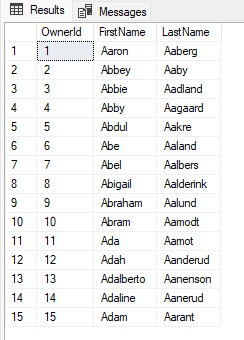
\includegraphics[width=0.6\linewidth]{Prt sc/Figure_1.jpg}  
		\end{minipage}
		\caption{Таблиця 'Ownerss'}
	\end{figure}

	\begin{figure}[h!]
		\centering
		\begin{minipage}[h]{1\linewidth}
			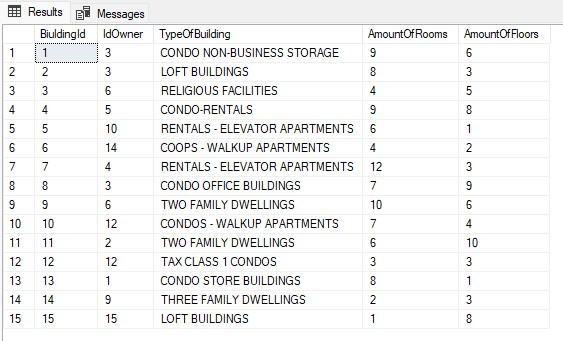
\includegraphics[width=0.8\linewidth]{Prt sc/Figure_2.jpg}  
		\end{minipage}
		\caption{Таблиця 'Building'}
	\end{figure}
	
	\begin{figure}[h!]
		\centering
		\begin{minipage}[h]{1\linewidth}
			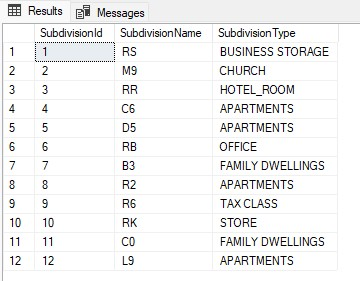
\includegraphics[width=0.8\linewidth]{Prt sc/Figure_3.jpg}  
		\end{minipage}
		\caption{Таблиця 'Subdivision'}
	\end{figure}

\newpage
	\begin{figure}[h!]
		\centering
		\begin{minipage}[h]{1\linewidth}
			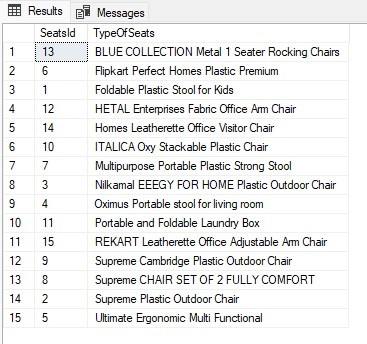
\includegraphics[width=0.8\linewidth]{Prt sc/Figure_4.jpg}  
		\end{minipage}
		\caption{Таблиця 'TypeOfSeats'}
	\end{figure}
	
	\begin{figure}[h!]
		\centering
		\begin{minipage}[h]{1\linewidth}
			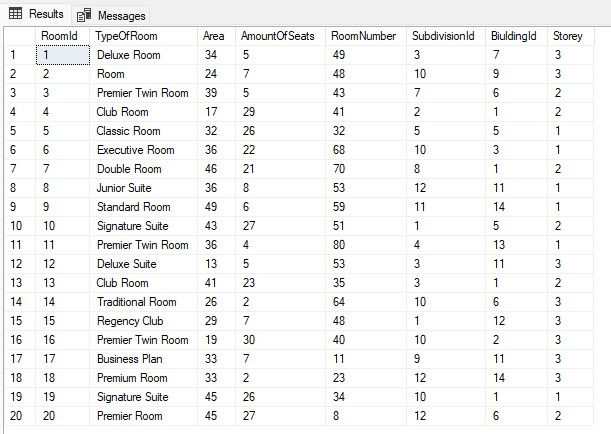
\includegraphics[width=0.8\linewidth]{Prt sc/Figure_5.jpg}  
		\end{minipage}
		\caption{Таблиця 'Room'}
	\end{figure}
	
	\begin{figure}[h!]
		\centering
		\begin{minipage}[h]{1\linewidth}
			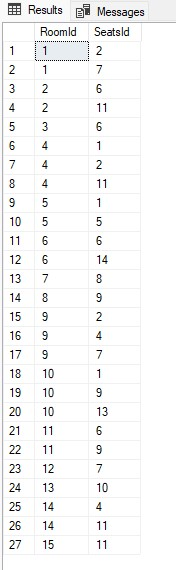
\includegraphics[width=0.4\linewidth]{Prt sc/Figure_6.jpg}  
		\end{minipage}
		\caption{Таблиця 'RoomSeats'}
	\end{figure}

\end{document}